% SC1004 Chapter 8: Eigenvalues, Eigenvectors & Diagonalization (0->100 ground-up)
\chapter{Eigenvalues, Eigenvectors, and Diagonalization}
\label{ch:eigen}

\begin{quote}
\emph{``Eigenvectors are the directions a matrix leaves alone --- it only stretches them.''} Finding those directions turns a tangled linear map into independent scalings, powers into powers of scalars, and differential equations into decoupled ones.
\end{quote}

\noindent\fbox{\parbox{\dimexpr\linewidth-2\fboxsep-2\fboxrule}{%
\textbf{From zero: fixed directions before polynomials.} We start with ``which arrows stay on their own span?'' then derive $A\mathbf{v}=\lambda\mathbf{v}$, the characteristic polynomial, and diagonalization. No prior eigen theory assumed.}}
\vspace{0.4em}

\section*{Learning Outcomes}
After this chapter you will be able to:
\begin{enumerate}[label=(L\arabic*)]
    \item define eigenvalue/eigenvector and find them via $\det(A-\lambda I)=0$;
    \item compute eigenspaces and their dimensions (geometric multiplicity);
    \item test diagonalizability and construct $A=PDP^{-1}$ when possible;
    \item use diagonalization to compute $A^k$, recurrences, and matrix exponentials;
    \item recognise symmetric matrices' orthogonal diagonalization and the spectral picture.
\end{enumerate}

% ============================================================
\section{Eigenpairs: Directions That Stay Put}
\label{sec:eigen-def}
A nonzero $\mathbf{v}$ is an \emph{eigenvector} of $A\in\mathbb{R}^{n\times n}$ with \emph{eigenvalue} $\lambda\in\mathbb{R}$ (or $\mathbb{C}$) if
\[
  A\mathbf{v}=\lambda\mathbf{v}.
\]
Geometrically, $A$ stretches $\mathbf{v}$ by $\lambda$ but does not rotate it off its line. $\mathbf{0}$ is never an eigenvector (but $\lambda=0$ is allowed --- then $A\mathbf{v}=\mathbf{0}$).

\begin{figure}[h]
\centering
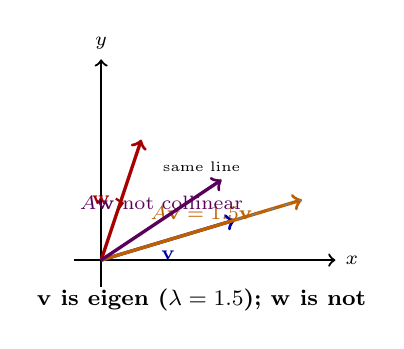
\begin{tikzpicture}[scale=0.85,every node/.style={font=\scriptsize}]
  \draw[->,thick] (-0.4,0)--(3.5,0) node[right] {$x$};
  \draw[->,thick] (0,-0.4)--(0,3.0) node[above] {$y$};
  \draw[->,very thick,blue!65!black] (0,0)--(2.0,0.6) node[midway,below] {$\mathbf{v}$};
  \draw[->,very thick,orange!75!black] (0,0)--(3.0,0.9) node[midway,above] {$A\mathbf{v}=1.5\mathbf{v}$};
  \draw[dashed,gray] (2.0,0.6)--(3.0,0.9);
  \node[font=\tiny,fill=white] at (1.5,1.4) {same line};
  \draw[->,very thick,red!65!black] (0,0)--(0.6,1.8) node[midway,left] {$\mathbf{w}$};
  \draw[->,very thick,violet!70!black] (0,0)--(1.8,1.2) node[midway,above] {$A\mathbf{w}$ not collinear};
  \draw[thick,red!60!black] (0.25,0.75)--(0.32,0.85)--(0.22,0.92);
  \node[font=\footnotesize\bfseries] at (1.5,-0.6) {$\mathbf{v}$ is eigen ($\lambda=1.5$); $\mathbf{w}$ is not};
\end{tikzpicture}
\caption{An eigenvector stays on its span under $A$; a generic vector is rotated off. The eigenvalue is the stretch factor (negative flips).}
\label{fig:eigen-direction}
\end{figure}

If $A\mathbf{v}=\lambda\mathbf{v}$ then $(A-\lambda I)\mathbf{v}=\mathbf{0}$ with $\mathbf{v}\neq\mathbf{0}$, so $A-\lambda I$ is singular. Hence

\begin{theorem}[Characteristic equation]
$\lambda$ is an eigenvalue of $A$ iff
\[
  p_A(\lambda)=\det(A-\lambda I_n)=0.
\]
$p_A$ is the \emph{characteristic polynomial} (degree $n$, leading term $(-\lambda)^n$ or $\lambda^n$ up to sign). Its roots are the eigenvalues; $\mathcal{N}(A-\lambda I)$ is the \emph{eigenspace} $E_\lambda$.
\end{theorem}

For $2\times2$, $A=\begin{bmatrix}a&b\\c&d\end{bmatrix}$,
\[
  p_A(\lambda)=\lambda^2-\operatorname{tr}(A)\lambda+\det(A),\quad \operatorname{tr}=a+d.
\]
So eigenvalues satisfy $\lambda_1+\lambda_2=\operatorname{tr}A$, $\lambda_1\lambda_2=\det A$ --- quick checks.

\begin{example}[A $2\times2$ shear vs.\ scaling]
$A=\begin{bmatrix}2&1\\0&3\end{bmatrix}$: $p_A(\lambda)=(2-\lambda)(3-\lambda)$, so $\lambda=2,3$. For $\lambda=2$, $(A-2I)=\begin{bmatrix}0&1\\0&1\end{bmatrix}$, $E_2=\operatorname{span}\{[1,0]^T\}$. For $\lambda=3$, $E_3=\operatorname{span}\{[1,1]^T\}$. Two independent eigen-directions --- diagonalizable (see \S\ref{sec:diag}).
\end{example}

\section{Eigenspaces and Multiplicities}
\label{sec:eigenspaces}
\emph{Algebraic multiplicity} $a_\lambda$: multiplicity of $\lambda$ as a root of $p_A$. \emph{Geometric multiplicity} $g_\lambda=\dim\mathcal{N}(A-\lambda I)$: number of independent eigenvectors for $\lambda$. Always $1\le g_\lambda\le a_\lambda$. Eigenvectors for distinct $\lambda$ are independent --- so $n$ distinct eigenvalues guarantees $n$ independent eigenvectors.

\begin{figure}[h]
\centering
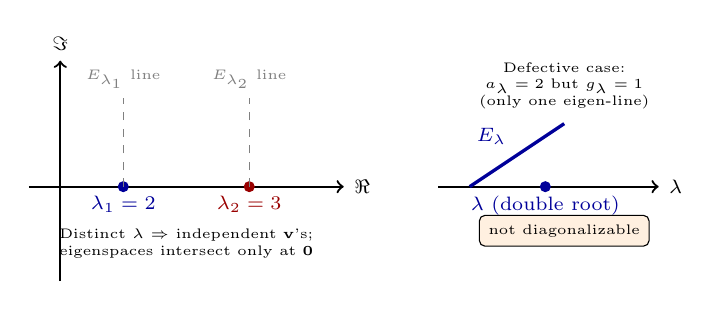
\begin{tikzpicture}[scale=0.80,every node/.style={font=\scriptsize}]
  \draw[->,thick] (-0.5,0)--(4.5,0) node[right] {$\Re$};
  \draw[->,thick] (0,-1.5)--(0,2.0) node[above] {$\Im$};
  \fill[blue!60!black] (1.0,0) circle (2.5pt) node[below] {$\lambda_1=2$};
  \fill[red!60!black] (3.0,0) circle (2.5pt) node[below] {$\lambda_2=3$};
  \draw[dashed,gray] (1.0,0)--(1.0,1.4) node[above,font=\tiny,fill=white] {$E_{\lambda_1}$ line};
  \draw[dashed,gray] (3.0,0)--(3.0,1.4) node[above,font=\tiny,fill=white] {$E_{\lambda_2}$ line};
  \node[font=\tiny,align=center] at (2.0,-0.9) {Distinct $\lambda$ $\Rightarrow$ independent $\mathbf{v}$'s;\\eigenspaces intersect only at $\mathbf{0}$};
  \begin{scope}[xshift=6.5cm]
    \draw[->,thick] (-0.5,0)--(3.0,0) node[right] {$\lambda$};
    \node[font=\tiny,align=center] at (1.5,1.6) {Defective case:\\$a_\lambda=2$ but $g_\lambda=1$\\(only one eigen-line)};
    \draw[very thick,blue!60!black] (0,0)--(1.5,1.0) node[midway,above left] {$E_\lambda$};
    \fill[blue!60!black] (1.2,0) circle (2.5pt) node[below] {$\lambda$ (double root)};
    \node[font=\tiny,fill=orange!12,draw,rounded corners=2pt] at (1.5,-0.7) {not diagonalizable};
  \end{scope}
\end{tikzpicture}
\caption{Left: distinct eigenvalues give independent eigenspaces. Right: a repeated eigenvalue may have fewer eigenvectors than its algebraic multiplicity --- defective, not diagonalizable.}
\label{fig:eigenspaces-mult}
\end{figure}

\begin{example}[Defective]
$J=\begin{bmatrix}2&1\\0&2\end{bmatrix}$ has $p_J(\lambda)=(2-\lambda)^2$, so $a_2=2$, but $J-2I=\begin{bmatrix}0&1\\0&0\end{bmatrix}$ has nullity $1$, so $g_2=1<2$. Only one eigen-line --- $J$ is not diagonalizable (it is a Jordan block).
\end{example}

\section{Diagonalization}
\label{sec:diag}
$A$ is \emph{diagonalizable} if $A=PDP^{-1}$ with $D=\operatorname{diag}(\lambda_1,\dots,\lambda_n)$ and $P$ invertible. Columns of $P$ are then eigenvectors and diagonal entries are the corresponding eigenvalues.

\begin{theorem}[Diagonalization criterion]
$A\in\mathbb{R}^{n\times n}$ diagonalizable $\iff$ there are $n$ linearly independent eigenvectors $\iff$ for every $\lambda$, $g_\lambda=a_\lambda$ (equivalently $\sum_\lambda g_\lambda=n$).
\end{theorem}

Why care? Powers decouple: $A^k=PD^kP^{-1}=P\operatorname{diag}(\lambda_1^k,\dots,\lambda_n^k)P^{-1}$. So does $e^{At}=Pe^{Dt}P^{-1}$ and linear recurrences $\mathbf{x}_{k+1}=A\mathbf{x}_k$.

\begin{figure}[h]
\centering
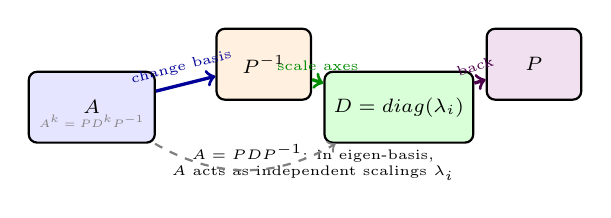
\begin{tikzpicture}[scale=0.78,every node/.style={font=\scriptsize}]
  \node[draw,thick,rounded corners=3pt,fill=blue!10,minimum width=1.6cm,minimum height=0.9cm] (A) at (0,0) {$A$};
  \node[draw,thick,rounded corners=3pt,fill=orange!12,minimum width=1.2cm,minimum height=0.9cm] (Pinv) at (2.8,0.7) {$P^{-1}$};
  \node[draw,thick,rounded corners=3pt,fill=green!15,minimum width=1.6cm,minimum height=0.9cm] (D) at (5.0,0) {$D=\operatorname{diag}(\lambda_i)$};
  \node[draw,thick,rounded corners=3pt,fill=violet!12,minimum width=1.2cm,minimum height=0.9cm] (P) at (7.2,0.7) {$P$};
  \draw[->,very thick,blue!60!black] (A)--(Pinv) node[midway,above,sloped,font=\tiny] {change basis};
  \draw[->,very thick,green!55!black] (Pinv)--(D) node[midway,above,font=\tiny] {scale axes};
  \draw[->,very thick,violet!60!black] (D)--(P) node[midway,above,sloped,font=\tiny] {back};
  \node[font=\tiny,align=center] at (3.6,-0.9) {$A=PDP^{-1}$: in eigen-basis,\\$A$ acts as independent scalings $\lambda_i$};
  \draw[->,thick,gray,dashed] (A) to[out=-30,in=-150] (D) node[midway,below,font=\tiny] {$A^k=PD^kP^{-1}$};
\end{tikzpicture}
\caption{Diagonalization as change of basis: $P^{-1}$ moves to eigen-coordinates, $D$ scales each axis by $\lambda_i$, $P$ moves back. Powers act entrywise on $D$.}
\label{fig:diagonalization}
\end{figure}

\begin{example}[Fibonacci via diagonalization]
$\begin{bmatrix}F_{k+1}\\F_k\end{bmatrix}=\begin{bmatrix}1&1\\1&0\end{bmatrix}\begin{bmatrix}F_k\\F_{k-1}\end{bmatrix}$, so $\mathbf{x}_k=A^k\mathbf{x}_0$. $A$ has eigenvalues $\varphi=(1+\sqrt5)/2$, $\psi=(1-\sqrt5)/2$, $A=P\operatorname{diag}(\varphi,\psi)P^{-1}$, giving $F_k=(\varphi^k-\psi^k)/\sqrt5$.
\end{example}

\begin{example}[Python --- eigen and diagonalization]
\begin{lstlisting}[language=Python]
import numpy as np
A = np.array([[2.,1.],[0.,3.]])
w, V = np.linalg.eig(A)          # w eigenvalues, V columns are eigenvectors
print(w)                          # [2., 3.]
print(A @ V[:,0], w[0]*V[:,0])   # check A v = lambda v
# Diagonalization check:
P = V
D = np.diag(w)
print(np.allclose(A, P @ D @ np.linalg.inv(P)))
# Powers:
print(np.allclose(np.linalg.matrix_power(A, 5), P @ np.diag(w**5) @ np.linalg.inv(P)))
\end{lstlisting}
For symmetric $A$, \texttt{eigh} returns orthonormal $Q$ with $A=Q\Lambda Q^T$ (spectral theorem).
\end{example}

\section{Symmetric Matrices and the Spectral Theorem}
\label{sec:spectral}
If $A^T=A$ (real symmetric), then all eigenvalues are real, eigenvectors for distinct $\lambda$ are orthogonal, and $A$ is orthogonally diagonalizable: $A=Q\Lambda Q^T$ with $Q^TQ=I$, $\Lambda$ real diagonal. This is the \emph{spectral theorem} --- the basis that diagonalizes a symmetric matrix is a rotation/reflection. Applications: PCA (covariance is symmetric), graph Laplacians, quadratic forms $Q(\mathbf{x})=\mathbf{x}^TA\mathbf{x}=\sum\lambda_i y_i^2$.

% ============================================================

% --- Additional depth: Complex eigenvalues, Markov, and SVD preview ---
\section{Complex Eigenvalues and Real Blocks}
\label{sec:complex-eigen}
Real matrices can have complex eigenpairs when they rotate. $R_\theta=\begin{bmatrix}\cos\theta&-\sin\theta\\\sin\theta&\cos\theta\end{bmatrix}$ has $\lambda=e^{\pm i\theta}$, eigenvectors $[1,\mp i]^T$ in $\mathbb{C}^2$. Over $\mathbb{R}$, $R_\theta$ is not diagonalizable but block-diagonalizable with $2\times2$ rotation blocks. The real Schur form captures this; the complex Schur form is always triangular.

\section{Markov Chains and Steady States}
\label{sec:markov}
A column-stochastic $P$ (nonnegative, columns sum to $1$) has $\lambda=1$ as its largest eigenvalue (Perron--Frobenius); the eigenvector $\pi$ with $P\pi=\pi$ is the \emph{steady state}. Powers $P^k\mathbf{x}_0\to\pi$ when $P$ is primitive ($|\lambda_2|<1$). Example: PageRank is the $\lambda=1$ eigenvector of the web's link matrix.

\begin{example}[Two-state chain]
$P=\begin{bmatrix}0.9&0.2\\0.1&0.8\end{bmatrix}$: eigenvalues $1,0.7$, $E_1=\operatorname{span}\{[2,1]^T\}$, so $\pi=[2/3,1/3]^T$ after normalising to sum $1$. Starting from any distribution, $P^k\mathbf{x}_0\to\pi$ at rate $0.7^k$.
\end{example}

\section{Singular Value Decomposition}
\label{sec:svd}
Every $A\in\mathbb{R}^{m\times n}$ factors as $A=U\Sigma V^T$ with $U,V$ orthogonal and $\Sigma$ diagonal holding \emph{singular values} $\sigma_1\ge\sigma_2\ge\cdots\ge0$, where $\sigma_i=\sqrt{\lambda_i(A^TA)}$. Intuition: every linear map is rotate--stretch--rotate---$V^T$ aligns the input axes, $\Sigma$ stretches, $U$ orients the outputs. Unlike eigen-decomposition, SVD exists for every matrix, even rectangular ones.
\begin{example}[Worked $2\times2$]
$A=\begin{bmatrix}3&0\\0&-1\end{bmatrix}$ is diagonal in disguise: $A^TA=\operatorname{diag}(9,1)$, so $\sigma_1=3,\sigma_2=1$ with $V=I$ and $U=\operatorname{diag}(1,-1)$ absorbing the sign. The unit circle maps to an ellipse with semi-axes $3,1$---singular values are exactly the stretch factors.
\end{example}
The count of nonzero $\sigma_i$ equals $\operatorname{rank}A$. Dropping small $\sigma_i$ gives the best low-rank approximation (Eckart--Young): this is PCA---keep the top principal stretches, discard the noise. If $A=Q\Lambda Q^T$ is symmetric, $\sigma_i=|\lambda_i|$.



\begin{remark}[Diagonalizability vs.\ invertibility]
These are unrelated: $\begin{bmatrix}0&1\\0&0\end{bmatrix}$ is singular and not diagonalizable; $\begin{bmatrix}1&1\\0&1\end{bmatrix}$ is invertible but not diagonalizable; $I$ is both. Test diagonalizability via $g_\lambda=a_\lambda$, not via $\det$.
\end{remark}

\begin{example}[Quadratic forms]
For symmetric $A=Q\Lambda Q^T$, $f(\mathbf{x})=\mathbf{x}^TA\mathbf{x}=\sum\lambda_i y_i^2$ where $\mathbf{y}=Q^T\mathbf{x}$. So $\lambda_i>0$ for all $i$ $\iff$ $f(\mathbf{x})>0$ for $\mathbf{x}\neq\mathbf{0}$ (positive definite) --- Ch.~6's $A^TA$ is always positive semidefinite ($\lambda_i\ge0$).
\end{example}



\begin{example}[Power iteration intuition]
Repeatedly applying $A$ to any $\mathbf{x}_0$ with a component in the dominant eigenspace amplifies the largest $|\lambda|$ direction fastest: $A^k\mathbf{x}_0\approx c_1\lambda_1^k\mathbf{v}_1$. Normalising each step gives the \emph{power method} for $\lambda_1,\mathbf{v}_1$ --- how PageRank and PCA's top component are found when $n$ is huge and full \texttt{eig} is too costly.
\end{example}


\section{Chapter Notes}
Eigen (German ``own'') --- Hilbert's term for characteristic values. Diagonalization fails exactly on nontrivial Jordan blocks; over $\mathbb{C}$ every matrix is triangularizable (Schur) and Jordan-form. Numerically, eigenvalues are found via $QR$ iteration (Francis, 1961), not $\det(A-\lambda I)$.

% ============================================================
\section{Exercises}
\label{sec:ch08-exercises}
\begin{enumerate}[label=E8.\arabic*, leftmargin=*, itemsep=0.8em]
\item \textbf{Find eigenpairs.} Compute eigenvalues and eigenspaces for $A=\begin{bmatrix}4&2\\1&3\end{bmatrix}$ via $p_A(\lambda)=\lambda^2-7\lambda+10$. Give eigenvectors and verify $A\mathbf{v}=\lambda\mathbf{v}$.
\item \textbf{Diagonalize or not?} For $B=\begin{bmatrix}2&1&0\\0&2&0\\0&0&3\end{bmatrix}$, find $a_\lambda,g_\lambda$ for each $\lambda$. Is $B$ diagonalizable? If so give $P,D$; if not explain why.
\item \textbf{Powers.} Let $A=\begin{bmatrix}1&2\\2&1\end{bmatrix}=PDP^{-1}$ with $D=\operatorname{diag}(3,-1)$. Compute $A^4$ via $PD^4P^{-1}$ and verify by direct multiplication.
\item \textbf{Symmetric.} Show $S=\begin{bmatrix}2&1&1\\1&2&1\\1&1&2\end{bmatrix}$ is symmetric, find its eigenvalues ($4,1,1$) and an orthonormal eigenbasis. Write $S=Q\Lambda Q^T$ and $\mathbf{x}^TS\mathbf{x}$ in $y=Q^T\mathbf{x}$ coordinates.
\item \textbf{Coding.} For random symmetric $5\times5$ $A=(M+M^T)/2$, use \texttt{np.linalg.eigh} to get $Q,\Lambda$ and verify $Q^TQ\approx I$, $A\approx Q\Lambda Q^T$, and $\det A\approx\prod\lambda_i$, $\operatorname{tr}A\approx\sum\lambda_i$ numerically.
\end{enumerate}
% End of Chapter 8
